\section{Branch and Bound method}
The Branch and Bound method employs a divide and conquer strategy to address ILP problems by systematically exploring the set of feasible solutions.
Let $F$ represent the set of feasible solutions for the problem:
\begin{align*}
    \min                    \:&\: c^T     \\
    \textnormal{such that }   &   x \in F \\
\end{align*}
The method unfolds in two main phases:
\begin{enumerate}
    \item \textit{Branch}: the problem is partitioned into simpler subproblems.
    \item \textit{Bound}: the subproblems are solved, and the optimal solution is determined.
\end{enumerate}
These two phases are applied recursively until a solution is discovered. 
If a problem remains unsolved during the bound phase, it is branched again until it becomes simple enough to find a solution. 
It's worth noting that this technique is applicable to a broad spectrum of problems, not exclusively limited to ILP problems.

\paragraph*{Branching}
The set of solutions $F$ is divided into $k$ disjoint subsets:
\[ F = F_1 \cup,  \ldots,  \cup F_k \quad F_i \cap F_j = \emptyset \: \forall,  i \neq j \]
Let $z_i$ be defined as:
\[ z_i = \min\left\{ c(x), \middle\vert, x \in F_i \right\} \quad i = 1,,  \ldots,  , k \]
The solution $z$ is then determined as:
\[ z = \min\left\{ c(x), \middle\vert, c \in F \right\} = \min\left\{ z_i,,  \ldots, , z_k \right\} \]

\paragraph*{Bounding}
For each subproblem $\min\left\{ c(x), \middle\vert, x \in F_i \right\}$, whose solution is found in the partition of $F$, the optimal solution $z_i$ is determined by either:
\begin{enumerate}
    \item Finding an optimal solution for $\min\left\{ c(x), \middle\vert, x \in F_i \right\}$.
    \item Proving that $F_i = \emptyset$.
    \item Proving that $z_i \geq z$, where $z$ is the optimal solution of the original problem found so far.
\end{enumerate}
If the subproblem is not resolved, it is necessary to generate a new subproblem by branching it again.

\paragraph*{Generic Branch and Bound Method}
If the lower bound $b(F_i)$ of the optimal solution for the subproblem $\min\left\{ c(x), \middle\vert, x \in F_i \right\}$ is greater than the optimal solution $z$ found so far, the subproblem is discarded, as it cannot contain a better solution than the one found so far.
At any point, the algorithm keeps in memory a set of active subproblems and the cost $U$ of the best feasible solution found so far.
Initially, $U$ is either $\infty$ or the cost of the best feasible solution found by the heuristic method (if any).
A typical step of the algorithm is:
\begin{enumerate}
    \item Select an active subproblem $F_i$ to be solved. 
    \item If the subproblem is infeasible, delete it; otherwise, compute $b(F_i)$ for the corresponding subproblem.
    \item If $b(F_i) \geq U$, delete $F_i$.
    \item If $F_i$ is feasible and $b(F_i) < U$, either:
        \begin{itemize}
            \item Obtain an optimal solution to the subproblem.
            \item Break the corresponding subproblem into further subproblems, which are added to the set of active subproblems.
        \end{itemize}
\end{enumerate}
There are several parameters that can be arbitrarily chosen. 
There is no fixed rule for many of them, as the best choice depends on the problem to be solved:
\begin{enumerate}
    \item There are multiple ways of choosing an active subproblem.
    \item There are multiple ways of breaking a subproblem into further subproblems.
    \item There are multiple ways of computing the lower bound $b(F_i)$.
\end{enumerate}

\subsection{Branching Tree}
The branching tree serves as a visual depiction of the branching progression within the Integer Linear Programming (ILP) problem. 
Each node in this tree corresponds to a subproblem derived from the larger ILP problem, and the edges symbolize the steps taken in the branching process.
Notably, a branching tree may not encompass all conceivable nodes or all potential leaves, which amount to $2^d$. 
A node in the tree is considered "fathomed" (having no child) under the following conditions:
\begin{enumerate}
    \item The initial constraint, along with those on the arcs from the root to the node, renders the subproblem infeasible.
    \item The optimal solution of the linear relaxation is an integer.
    \item The value $C^T \overline{x}_{\text{LP}}$ of the optimal solution $\overline{x}_{\text{LP}}$ from the linear relaxation is inferior to the best feasible solution $z$ discovered thus far.
\end{enumerate}
This set of criteria, termed the branching criterion, enables the exclusion of numerous nodes (representing subproblems) that would not contribute to a valid solution, thereby curtailing the size of the tree.
\begin{figure}[H]
    \centering
    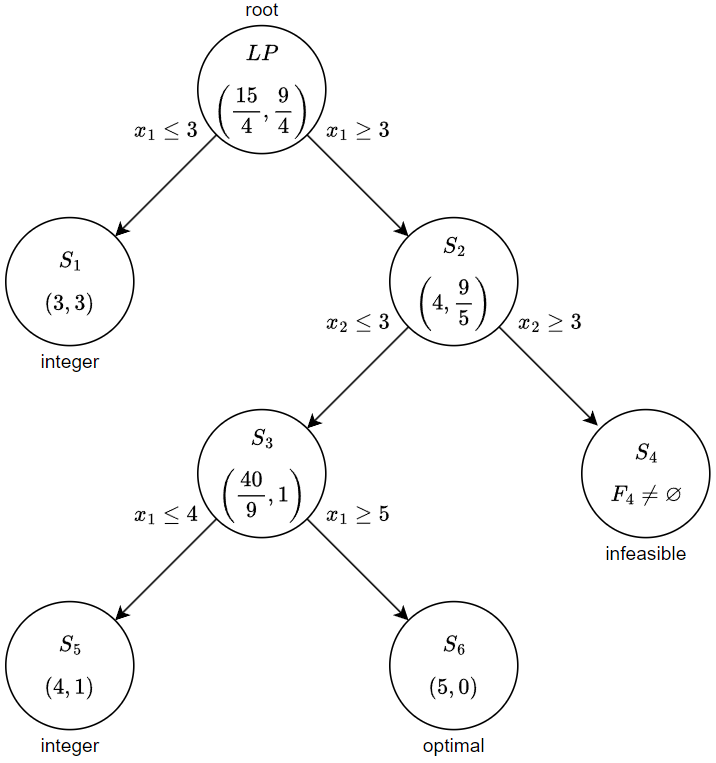
\includegraphics[width=0.5\linewidth]{images/ilp3.png}
    \caption{Branching tree}
\end{figure}

\subsection{Branch and Bound for the ILP problem}
In the context of an Integer Linear Programming (ILP) problem given by:
\[ \min\left\{ c^T x, \mid, Ax = b, \ x \in \mathbb{N} \right\} \]
the Branch and Bound method proves to be an effective strategy for determining the optimal solution $z$.

\paragraph*{Branching}
The first step involves partitioning the feasible region $F$. 
Let $\overline{x}$ represent an optimal solution of the linear relaxation of the ILP:
\[ \min\left\{ c^T x, \mid, Ax = b, \ x \geq 0, \ x \in \mathbb{R} \right\} \quad z_{\text{LP}} = c^T \overline{x} \]
If $\overline{x}$ is an integer, it serves as the optimal solution for the ILP problem. 
However, if $\overline{x}$ is non-integer, the ILP is divided into two subproblems:
\[\min\left\{ c^T x, \middle\vert, Ax = b, x \leq \left\lfloor \overline{x} \right\rfloor \right\} \label{eq:branch1}\]
\[\min\left\{ c^T x, \middle\vert, Ax = b, x \geq \left\lceil \overline{x} \right\rceil \right\} \label{eq:branch2}\]
Here, $ \left\lfloor \overline{x} \right\rfloor $ and $ \left\lceil \overline{x} \right\rceil $ represent the floor and ceiling of the vector $\overline{x}$.
While choosing the variable $x_h$ closest to $0.5$ for branching can be a common approach, it may not always yield the best results.
An alternative and more effective strategy is strong branching, wherein candidate variables (specifically, fractional basic ones) are considered. 
Evaluation of the corresponding objective function values helps determine the variable that, upon branching, produces the most substantial improvement in the objective function value.

\paragraph*{Bounding}
The process of bounding involves determining a lower or upper bound on the optimal value $z_i$ of a subproblem within the Integer Linear Programming (ILP). 
The nature of the bound depends on whether the ILP is a minimization or maximization problem. 
This is achieved by solving the linear relaxation of the subproblem.
To decide which node (subproblem) to address next, the following criteria can be considered:
\begin{itemize}
    \item \textit{Deeper nodes first} (depth-first search strategy): this strategy selects the node with the greatest depth in the tree of subproblems. 
        While simple to implement and optimize, it may result in a large tree of subproblems if the branching variable is chosen incorrectly.
    \item \textit{More promising nodes first} (best-bound first strategy): this approach prioritizes the node with the best linear relaxation value $b(F_i)$. 
        Although it generates a smaller tree of subproblems, the subproblems are less constrained, leading to longer times to find a feasible solution and improve it.
\end{itemize}

\subsection{Remarks on the Branch and Bound method}
Branch and Bound extends its utility to mixed Integer Linear Programming (ILP) problems. During the branching step, treating fractional variables as integers and vice versa facilitates its application.

Initiating the method with a well-crafted initial feasible solution from a heuristic algorithm can enhance performance. 
This contributes to obtaining more accurate lower or upper bounds in the context of maximization or minimization problems, respectively.

As a versatile approach, Branch and Bound can serve as a heuristic method for ILP problem resolution, halting when the best feasible solution discovered surpasses the best integer solution identified thus far.

\paragraph*{Efficient solution of the linear relaxation}
Iteratively solving the linear relaxations of ILP subproblems from scratch at each branching step is unnecessary. 
The solution of the linear relaxation at the parent node can be utilized as a starting point for solving the linear relaxation at the child node.

Employing a single iteration of the Dual Simplex method (the simplex method applied to the dual problem) efficiently yields an optimal solution to the linear relaxation with an additional constraint. 
This optimization builds upon the optimal Branch and Bound outcome of the preceding node (linear relaxation of the parent subproblem).

\paragraph*{Applicability of Branch and Bound approach}
The applicability of the Branch and Bound method extends beyond discrete optimization problems to encompass numerous non-linear optimization challenges. 
However, adaptations are required in two key procedures:
\begin{itemize}
    \item The division of the feasible region into subregions (branching).
    \item The determination of a bound on the optimal value of the subproblem (bounding).
\end{itemize}